\chapter{Data}
\label{chap:data}

To better understand the optimisation and network limitations, it makes sense to explain how the data is produced, how it is organised, and how it can be applied. The data generation can largely be separated into CFD and Aeroelastic simulations. 

\section{CDF}

The CDF calculations are created through EllipSys3D, which computes wind data through Large Eddy Simulations. The necessary theory is briefly explained in \ref{sec:LES} and will not be elaborated further. The turbine used is an IEA10MW, a theoretical turbine used for research applications \cite{turbineref}. For the setup, we use 12 cases of the upstream turbine, modelled with an actuator disk approach \cite{actuatordisk}. We will consider only negative yawing angles as configurations go, as we know these to behave symmetrically from section \ref{dimensionless_power}. For pitching, we only consider positive or very slight negative angles since large negative angles were not beneficial, as determined in section \ref{dimensionless_thrust}. The 12 different combinations of control parameters are displayed in table \ref{table:configurations}.

\begin{table}[H]
\begin{tabular}{|c|c|c|c|c|c|c|c|c|c|c|c|c|}
\hline
Case nr. & 0    & 1    & 2    & 3    & 4    & 5    & 6    & 7    & 8    & 9    & 10   & 11   \\ \hline
Omega    & 0.75 & 0.75 & 0.75 & 0.75 & 0.75 & 0.75 & 0.75 & 0.87 & 0.76 & 0.84 & 0.68 & 0.81 \\ \hline
Pitch    & -0.5    & -0.5   & -0.5    & -0.5  & -0.5 & -0.5 & -0.5 & 2.06 & 1.38 & 1.30 & 3.44 & 2.88  \\ \hline
Yaw      & 0    & -5    & -10   & -15   & -20   & -25   & -30   & -15   & -20   & -25   & -15   & -20   \\ \hline
\end{tabular}
\caption{Configurations used in CDF simulations}
\label{table:configurations}
\end{table}

For each of these cases, the flow is captured at 28 different downstream distances one radius apart, starting at $0R$ and going up to $27R$. Additionally, the simulation is separated into 21 smaller periods to get a statistical groundwork for the somewhat unpredictable nature of the flow, with each separation containing 17501 data points, over a $700s$ period, for each of the three velocity components. 


\section{Aeroelastic}
\label{sec:Aeroelastic}

Regarding the Aeroelastic simulations, we are only concerned about the flow entering the turbine, which implies that the second turbine's wake is irrelevant. We, therefore, utilise a "ghost turbine" approach, in which the down steam turbine does not affect the flow and does not need to be included in the CFD simulations. The turbine's reaction to wind conditions is determined through Blade element theory, explained in \ref{sec:blademomentum}. What is especially important to realise is the computational gain through this method. Since we do not have to perform heavy CDF calculations for each two-turbine configuration, we can test a wide variety of yawing angles. This is important when training the surrogates, where the extra data is very beneficial. 

It is easy to imagine that there will be little to no benefit in yawing for very large spacings. It is also logical that alterations will not be efficient for very close distances since the turbines perform poorly under any circumstance. For this reason, it's interesting to investigate which distances yield the greatest benefit, if any, for this kind of optimisation. However, due to the project's time constraint, we can not evaluate this properly, and will therefore, temporarily assume that the turbines perform similarly to smaller turbines analysed in previous studies. A very recent paper \cite{charles} showed that the highest relative increase is seen at approximately $6R$, which will be the basis for the analysis. We will also look into a more standardised distance of $14R$ to see how this compares. For the second turbine yawing, we will investigate the following angles. 

\begin{equation*}
    s \in \{ 6R, 14R\}, \quad \psi_2 \in \{ -30^\circ,-28^\circ..28^\circ, 30^\circ \}
\end{equation*}

Note that these calculations must be performed for all 21 periods at each configuration, which results in massive data that needs to be modelled to lower the computational cost. This is done by collecting the average value of relevant parameters for each period, yielding 21 similar averages. Plotting these as a cumulative distribution function gives a familiar s-curve well-known for normally distributed quantities. To represent this as simply as possible, we will fit a Weibull curve to the cumulative distribution through maximum likelihood estimation \cite{maxlikelihood}. A randomly selected example of such fit is illustrated in figure \ref{fig:weibullexample}

\begin{figure}[H]
    \centering
    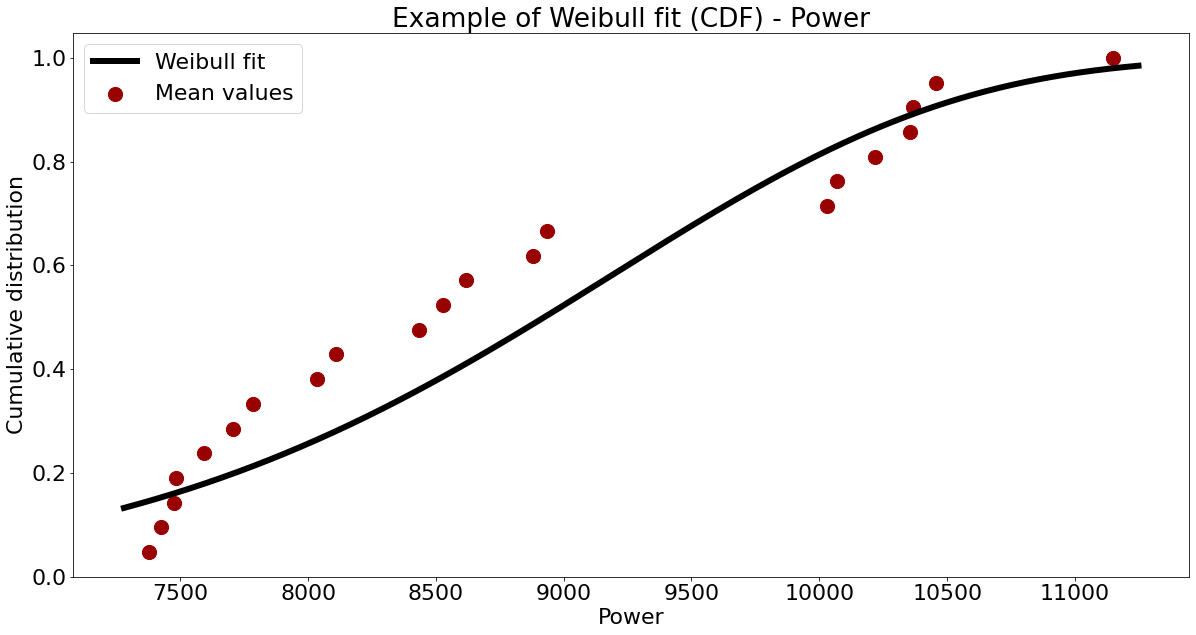
\includegraphics[scale=0.25]{Illustrations/weibullfitexample.png}
    \caption{Weibull fit on power CDF for $\psi_1 = 25^\circ, \; \theta_1 = -0.5^\circ, \; \Omega_1 = 0.75 \; m/s, \; \psi_2 = 15^\circ$}
    \label{fig:weibullexample}
\end{figure}

\section{Weibull}
\label{weibull}

A Weibull distribution is a continuous probability distribution widely used in probability theory. It can be expressed as both a probability density function (PDF) and a cumulative density function (CDF) and is defined by only two parameters, referred to as shape and scale. The CDF, being most relevant to the problem, is expressed as

\begin{equation}
Weibull_{CDF}(x)=\begin{cases}1-e^{-(x / \lambda)^k}, & x \geq 0 \\ 0, & x<0\end{cases}
\end{equation}

With $\lambda$ being the scale and $k$ being the shape. In theory, this heavily simplifies the data both in size and complexity, but we need to investigate if this is an accurate representation before applying it in the analysis. A good measure of such accuracy is the coefficient of determination, often referred to as the $R^2$ value. Although there are different definitions of $R^2$, the value is generally expressed as

\begin{equation}
R^2=1-\frac{\sum_i\left(y_i-f_i\right)^2}{\sum_i\left(y_i-\bar{y}\right)^2},
\end{equation}

where $f_i$ is the modelled probability and $y_i$ is the true value for the data. Since the fit accuracy will vary between runs, we should consider how the $R^2$-values are distributed. Plotting so yields the graph presented in figure \ref{fig:Rsquare}

\begin{figure}[H]
    \centering
    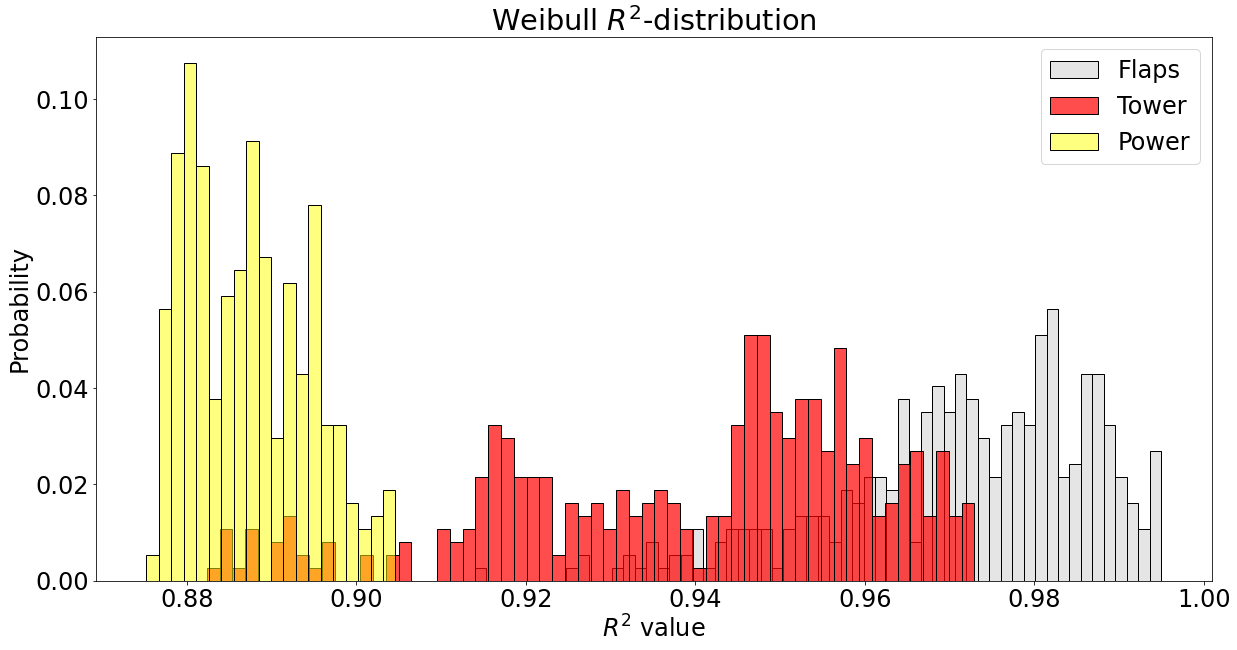
\includegraphics[scale=0.3]{Illustrations/R_2_values.png}
    \caption{$R^2$-value density distribution}
    \label{fig:Rsquare}
\end{figure}

Firstly we will note that even for the worst fit, which seems to deviate heavily from the mean, the model can still explain over $85\%$ of the variance within the data. An interesting trend is that power generally performs worse than loads. However, this is a small margin, and both would be considered highly correlated with the proposed fit. For further analysis, we will consider the Weibull constants an adequate representation of the data sets. When used for optimisation, it should be noted that none of these constants is directly applicable, and we should instead use both to compute another more useful measure. There are two obvious ways to represent this: the mean and median. Although it is difficult to answer which is better, we will apply the median with the argument that it is less sensitive to large individual fluctuations in the data. The median for Weibull distributions can be expressed as

\begin{equation}
    \mu = \lambda \ln (2)^{\frac{1}{k}}
\end{equation}

Additionally, we can express the uncertainty on the median as the standard deviation, which is expressed as

\begin{equation}
    \sigma = \lambda\sqrt{\Gamma\left(1+\frac{2}{k}\right)-\Gamma\left(1+\frac{1}{k}\right)^2}
\end{equation}

where $\Gamma()$ is the gamma function. By this logic, we can predict a turbine's expected power or load as $\mu \pm z \cdot \sigma$, where $z$ denotes the number of standard deviations. In the case of the final evaluation, we use $z=1$, which is the custom when applying standard deviation as uncertainties. 

